\documentclass{fpgairpods}
\usepackage[letterpaper, margin=1in]{geometry}

\addbibresource{report.bib}
\graphicspath{{figs/}}

\setlist{noitemsep, topsep=0pt}

\begin{document}

\title{\textit{FPGAirPods}: Implementing Active Noise Cancellation on a Xilinx Nexys7 FPGA}
\date{6.111 Introductory Digital Systems Laboratory \\ \textit{Massachusetts Institute of Technology} \\ \today}
\author{Ben Kettle \\ \ttt{bkettle@mit.edu} 
\and Nicholas Ramirez \\ \ttt{ramirezn@mit.edu} \and Gokul Kolady \\ \ttt{gokulk@mit.edu}}

\maketitle
\tableofcontents

\newpage
\begin{multicols}{2}
\section{Introduction and Motivation}

Noise cancellation is in demand. At the time of writing this, Apple has just released AirPods Max for \$550.

\section{Project Overview} % talk about how the system works right now, here is where we should put graphs of cancellation effectiveness at different frequencies
% I think we can generate those graphs by making a python script to analyze ILA output and give the average amplitude of the wave, then we just compare these to find a dB cancelled
Our 6.111 final project aimed to implement active noise cancellation as seen in over-ear and in-ear headphones such as the Bose QC35 and the AirPods Pro (hence the name). In order to do this, we first created a physical model of a single headphone (one ear cup) that we used to test. Inside the ear cup, we installed a speaker (far from the ear) and a feedback digital microphone (closer to the ear). In addition, we used a digital microphone external to the ear cup in order to capture ambient noise. To prevent feedback issues, we lined the inside of the model with

The FPGA itself handles the computational side of the active noise cancellation. The general flow of the system starts with sampling the incoming signal from the microphones, processing the samples, and outputting the anti-noise signal. We sample the microphones at a rate of 65 kHz which means our maximum target latency is 5830 clock cycles. 

The logic behind utilizing this sampling rate was to allow enough time for us to sample an outside signal from the ambient microphone, apply a filter to create the anti-noise signal, and output that anti-noise signal before the outside signal reaches the speaker. Since the ambient microphone is about 2 cm away from the speaker and noise travels around 332 meters per second, we have around 60.241 microseconds. 

For processing the samples, we used the Normalized Least Mean Squares (NLMS) adaptive filter to continually calculate coefficients that aim to minimize the error function --- i.e., the noise that makes it through and is not cancelled out. These updated coefficients are then applied to the input ambient sample by a Finite Impulse Response (FIR) filter and played out the speaker to cancel the noise. 

\end{multicols}

\begin{figure}
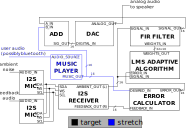
\includegraphics[width=\textwidth]{./figs/block_diagram.pdf}
\caption{The high-level block diagram for our system.}
\label{fig:blockdiagram}
\end{figure}

\newpage
\section{Hardware Testing Setup (Ben)}
\subsection{Testing Hardware (Ben)}
In order to demonstrate that our system was functional, a system to test on was crucial. This system would include the FPGA as a processing center with a variety of peripherals, as shown in Figure \ref{fig:peripherals}.

\begin{figure}[h]
\centering
\includegraphics[width=300pt]{./figs/system_diagram_with_text.pdf}
\caption{The peripherals that will be included in our project}
\label{fig:peripherals}
\end{figure}

\section{Implementation Details}
Our implementation was structured as a series of modules each applying some processing on the incoming ambient noise signal. We devised a common scheme for all these modules to share, where in addition to any other samples or signals it requires, each module includes a \ttt{ready_in} signal and outputs a \ttt{ready_out} signal---each 1 clock cycle long. This allows us to chain many of these modules together, feeding \ttt{done_out} of each into \ttt{ready_in} of the next.

\subsection{I2S Receiver (Ben)}
This module is the origin of the \ttt{ready_in} pulse chain described above---it implements the I2S protocol as described in the datasheet for the microphones we use\autocite{mic_datasheet}. In essence, this requires the creation of an \ttt{LRCLK} signal that controls whether the left (ambient) or right (feedback) mic will currently transmit. For every change of this clock, the corresponding microphone would begin sending a new sample. We drove this clock at the 4MHz, the maximum rate tolerated by the microphones, for a sampling rate through our system of 65 kHz.

\subsection{FIR Filter - \textit{Niko}}
The FIR Filter module convolves the external ambient noise with a set of filter coefficients in order to produce an anti-noise signal. Our module uses 64 taps

The filter calculation requires forming the following sum:

$$ y[n] = \sum_{i=0}^{63} (c_i * x[n-i]) $$



These coefficients are set continuously by the LMS adaptive algorithm module.
\subsubsection{Inputs}
\begin{itemize}
    \item \ttt{external_signal_in[15:0]}: The current sample from the external microphone that will be filtered.
    \item \ttt{weights_in[31:0][9:0]}: Coefficients that the filter will use for convolution.
\end{itemize}
\subsubsection{Outputs}
\begin{itemize}
    \item \ttt{antinoise_out[15:0]}: Anti-noise signal that will be used to cancel out ambient noise.
\end{itemize}
\subsubsection{Complexity/Level of Performance}
This module will be time sensitive, as we will want to calculate the output corresponding to a given input in very little time in order to enable effective noise cancellation. Because of this, we anticipate a significant amount of time to be spent streamlining the functionality of the filter module and improving its performance. As part of this, we need fast access to the previous samples to use for the convolution, so these previous samples from the external microphone will be stored in a circular buffer as a 32 element array with each element 16 bits wide. Implementing this as a BRAM would be to slow, so it will be implemented with distributed RAM. Some optimization that we are considering for this module is performing the additions in a tree structure rather than sequentially and streamlining the multiplications if necessary. We expect this to include 32 multiplications and 32 additions.

\subsubsection{Testing - \textit{Gokul}}
Testing for this module will consist of simple inputs similar to those seen in Lab 5a with known filter coefficients, such as a low pass filter with an impulse input, a sine input, etc. If these show the results that we expect, we can conclude that the FIR filter works. Later, we will also test it in conjunction with the LMS.

\subsection{LMS \& NLMS Adaptive Algs. - \textit{Gokul \& Niko}}
This module uses the LMS adaptive algorithm in order to update the coefficients of the FIR Filter for better noise cancellation. This algorithm takes advantage of the steepest descent optimization method, which analyzes the impact of the previous filter coefficients on the observed error and computes appropriate adjustments. This update is accomplished using the following equation\cite{lmsfilter}, where $b_k(n)$ is the FIR coefficient for a given $k$ value and a given timestep $n$, $\Lambda$ is a predefined step size or learning rate that defines how quickly the filter weights change, $e(n)$ is the calculated error, $f(n)$ is the value of the noise sample from the external microphone at a timestep $n$, and $M$ is the number of coefficients in the FIR filter:
\[ b_k(n + 1) = b_k(n) + \Lambda e(n)f(n-k) \]
\[ k = 0, 1, 2,\ldots,  M-1 \]

\subsubsection{Inputs}
\begin{itemize}
    \item \ttt{external_signal_in[15:0]}: The current sample from the external microphone (previous samples get used in weight update formula, so they must be stored in this module).
    \item \ttt{error_in[15:0]}: The error between the internal microphone signal and the desired signal.
\end{itemize}
\subsubsection{Outputs}
\begin{itemize}
    \item \ttt{weights_out[31:0][9:0]}: Updated coefficients to be used by the FIR filter in the next timestep for improved anti-noise generation.
\end{itemize}
\subsubsection{Complexity/Level of Performance}
To implement this operation, we will need to store the last $M$ noise inputs from the external microphone along with the full last set of filter coefficients. Previous samples from the external microphone will be stored in a circular buffer as a 32 element array each 16 bits wide, and the coefficients will be stored similarly in distributed RAM if possible, 32 elements each 10 bits wide.

\subsubsection{Testing - \textit{Niko}}
Testing this module will be a bit more involved than some of the others due to its not well-defined behavior, but in order to test the behavior we will need to have a working FIR module. With this module in place, we can then test the ability of the LMS algorithm to recreate the coefficients of a given filter. In other words, we can have our "desired" signal be the result of passing some input through an arbitrary filter, use this desired signal to calculate the error $e(n)$, and pass this error into our LMS module. If the input of the LMS module is the same as the input to this mystery filter, we can conclude that the LMS algorithm is functioning as necessary.

\subsection{Error Calculator - \textit{Gokul}}
The error calculator module monitors the error our system encounters in order to pass it into the NLMS. At first, this module's function was simply to negate the feedback microphone signal (post-processing) and hand it off to the NLMS algorithm, 

\subsubsection{Inputs}
\begin{itemize}
    \item \ttt{antinoise_in[15:0]}: One of the two signals to be added.
    \item \ttt{music_signal_in[15:0]}: The other signal to be added.
\end{itemize}
\subsubsection{Outputs}
\begin{itemize}
    \item \ttt{full_digital_signal_out[15:0]}: The sum of the two signals.
\end{itemize}

\subsection{DC Remover (Gokul)}
Early on in our project, we realized that both of the microphone signals that our system received were centered somewhere in around -1780 to -1830. Additionally, when playing a sine tone from our external speaker, we would occasionally notice a small low-frequency oscillation in the DC offset of the sine tone when picked up by the digital microphones. We realized that the former issue would cause our NLMS algorithm to take an unnecessary extra amount of time to converge, as it would first have to learn that the input is centered around some very low negative value before performing any meaningful learning regarding the nature of the input signal. As for the latter issue, we figured that these small oscillations in DC offset would likely cause the error in the system to waiver slightly even after convergence.

To account for these problems, we implemented a module that removes the DC offsets present in the microphone inputs in order to center these signals closer to 0. The module itself takes in raw samples from the I2S module (pre-lowpass) and outputs these samples with the average of the last 64 raw samples subtracted from them (this average being an approximation of DC offset based on recent input). The sum of the most recent 64 raw samples is maintained in a 22-bit variable, and the average is computed by extracting bits 21 though 6 of that sum variable, effectively dividing the sum by 64. One potential drawback of using this process to remove unwanted DC offset from our signal is that low frequencies are somewhat penalized, as every set of 64 samples is re-adjusted even though some of the offset present in these samples might be a product of the oscillations caused by these low frequencies. In other words, if cancellation of lower frequencies within input noise is desired, this module would likely need to be adjusted to accommodate them.

\subsection{Music Receiver (Ben)}
receives music

\subsection{Audio Mixing (Ben)}
mixes audio

\section{Challenges}
\subsection{Feedback}
Our initial hardware testbench did not include as much passive cancellation as our final design. When we tried 

\subsection{Microphone Noise}

\subsection{Choosing LMS Step Size Empirically}

\subsection{Instability of NLMS Convergence}

\subsection{Speaker Limitations}
In our testing, we noticed that the frequency response of our speaker was not flat, particularly at low frequencies. Include a graph here.

\section{Reflections and Recommendations}

\section{References}

\printbibliography

\end{document}
